\chapter{Preliminaries}
\label{chap:preliminaries}
Before delving into an overview of existing works in style transfer, it is crucial to clarify the terminology used in this field. Although "style transfer" and "stylization" often appear interchangeably in literature, they denote distinct concepts within the realms of 2D and 3D computer vision. These concepts will be explored in the following sections.

\section{Stylization, Style Transfer and similar concepts}

To begin, "style" is defined as a distinctive way an individual expresses creativity and authenticity \citep{Chen.2023}. In the 2D domain, style transfer refers to the process of imparting stylistic elements from one image to another. Stylization encompasses a broader spectrum, involving various transformations aimed at altering an image's aesthetic. The objective of image stylization is to create visually appealing images that embody specific artistic styles like impressionism or surrealism, without necessarily referencing another image, unlike style transfer.

\subsection{Style Transfer}

In contemporary research, style transfer is often equated with image-to-image translation (I2I), which transforms a content image to align with the style or characteristics of a reference image \citep{Pang.2021}. Neural networks, which separate content and style, typically achieve this transformation. Style transfer is often applied for artistic purposes, such as replicating the style of renowned artists or modifying image aesthetics while preserving content. In 3D, style transfer expands to include geometric style transfer (shape deformation) and texture style transfer (color transformation) \citep{Yin.2021}. Many works, including those cited in this thesis, use "style transfer" and "stylization" interchangeably due to the reliance on target style inputs, such as images or texts, applied to content.

\subsection{Editing vs Stylization}

Style transfer and stylization differ from editing. In 2D, image editing involves modifying content or style with strict constraints to preserve original characteristics and shapes. This includes tasks like color filtering, object masking, and quality enhancement (e.g., sharpening, deblurring) \citep{Jing.2020}. Similarly, 3D editing modifies geometry, appearance, or style, integrating classical 3D modeling techniques with neural networks \citep{Chen.2023}.

\subsection{NPR as stylization approach}

Non-Photorealistic Rendering (NPR) originated in computer graphics to render non-realistic images during post-processing. Today, NPR intersects with computer vision \citep{Rosin.2022}. Traditional NPR algorithms employ techniques like cel shading and stippling to emulate hand-drawn cartoons or pointillist paintings. However, these algorithms offer limited stylistic flexibility, requiring handcrafted patterns and heuristics \citep{Jing.2020}. With advancements in neural networks, researchers have pursued neural style transfer (NST) for more intelligent and automatic stylization \citep{Gatys.2015}.

In summary, editing encompasses various content and style alterations, including stylization. Style transfer is a subset of stylization that uses neural networks to apply one input's style to another. \Textcite{Johnson.2016} generalize these tasks as "image transformation tasks." NPR represents a specific algorithmic stylization approach, less flexible than neural-based methods and not typically classified as style transfer.

This thesis focuses on 3D Gaussian Splatting style transfer, aiming to develop a metric quantifying multi-view consistency between cameras and stylized 3D faces. The employed framework not only alters the 3D object's appearance based on target style but also adds details to the original model. Chapter \ref{chap:relatedwork} overviews the framework used, alongside relevant literature. Methodology and implementation specifics for obtaining and stylizing the 3D model are detailed in Chapter \ref{chap:method}.

\section{Various 3D Representations}

In computer graphics, a 3D model represents a three-dimensional object in digital form, capable of being stored and visualized on a computer. Geometric objects are categorized into explicit, implicit, and hybrid representations.

Explicit representations describe 3D objects using basic primitives (points, triangles), as seen in point clouds and meshes. Implicit representations, like Neural Radiance Fields (NeRFs) \citep{Mildenhall.2020}, encapsulate volumetric details, offering continuous and detailed modeling at the cost of slower optimization. Unlike explicit representations, which focus on object surfaces, implicit representations define an object's entire volume. Hybrid representations merge explicit and implicit strengths, balancing efficient optimization with flexible topology. Notable hybrids include voxel grids and triplanes. The following sections provide an overview of these representations, most relevant to this thesis.

\begin{figure}
    \centering
    \begin{subfigure}{0.48\linewidth}
        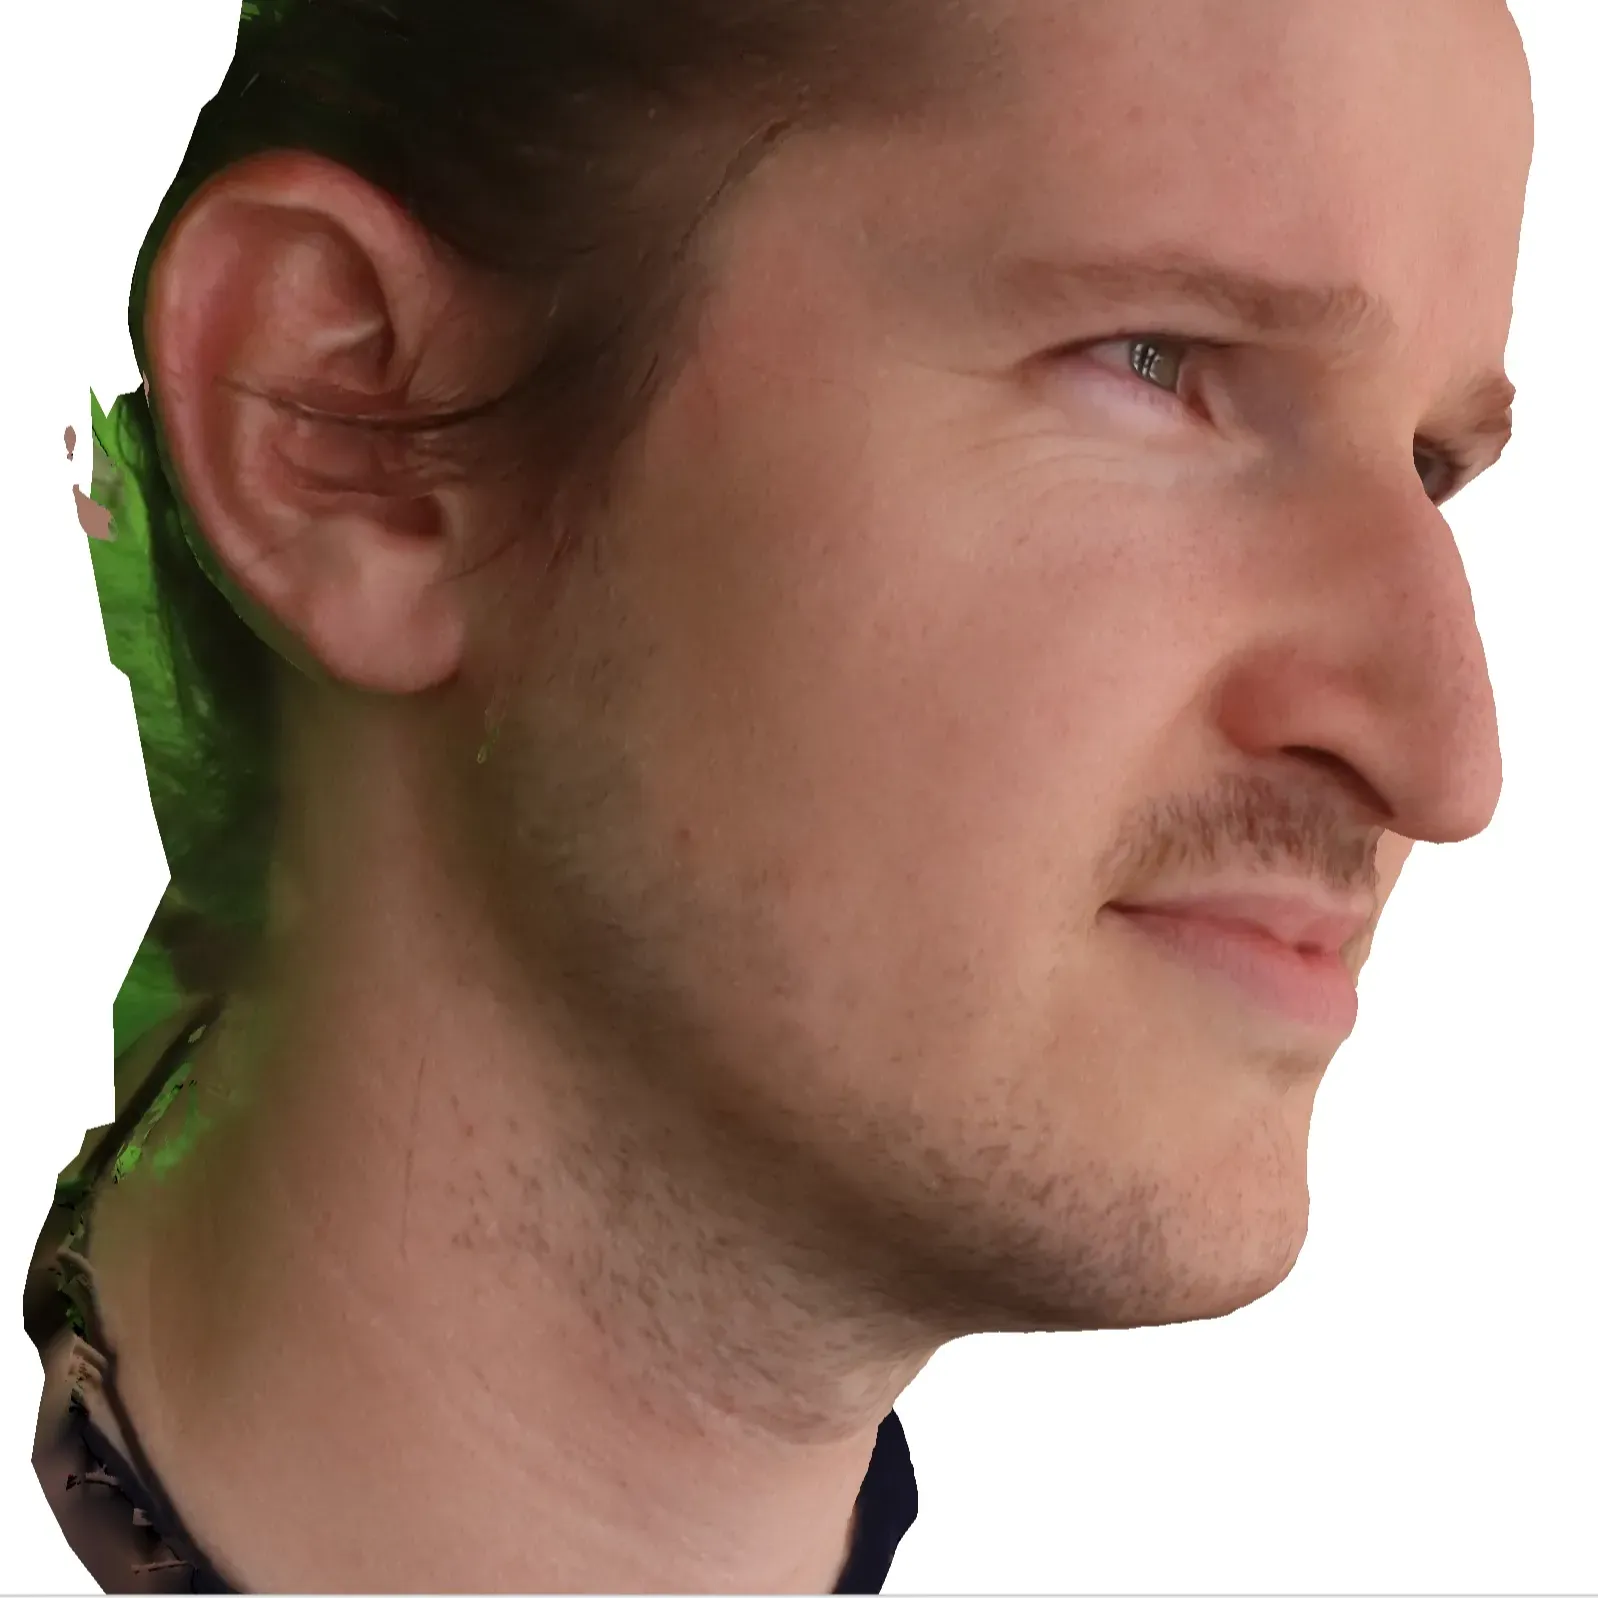
\includegraphics[width=\textwidth]{Figures/basics/rep2.png}
        \caption{Textured Mesh}
    \end{subfigure}
    \begin{subfigure}{0.48\linewidth}
        \includegraphics[width=\textwidth]{Figures/basics/rep1.png}
        \caption{Wireframe Mesh}
    \end{subfigure}
    \begin{subfigure}{0.48\linewidth}
        \includegraphics[width=\textwidth]{Figures/basics/rep3.png}
        \caption{Point Cloud (with accuracy level)}
    \end{subfigure}
    \begin{subfigure}{0.48\linewidth}
        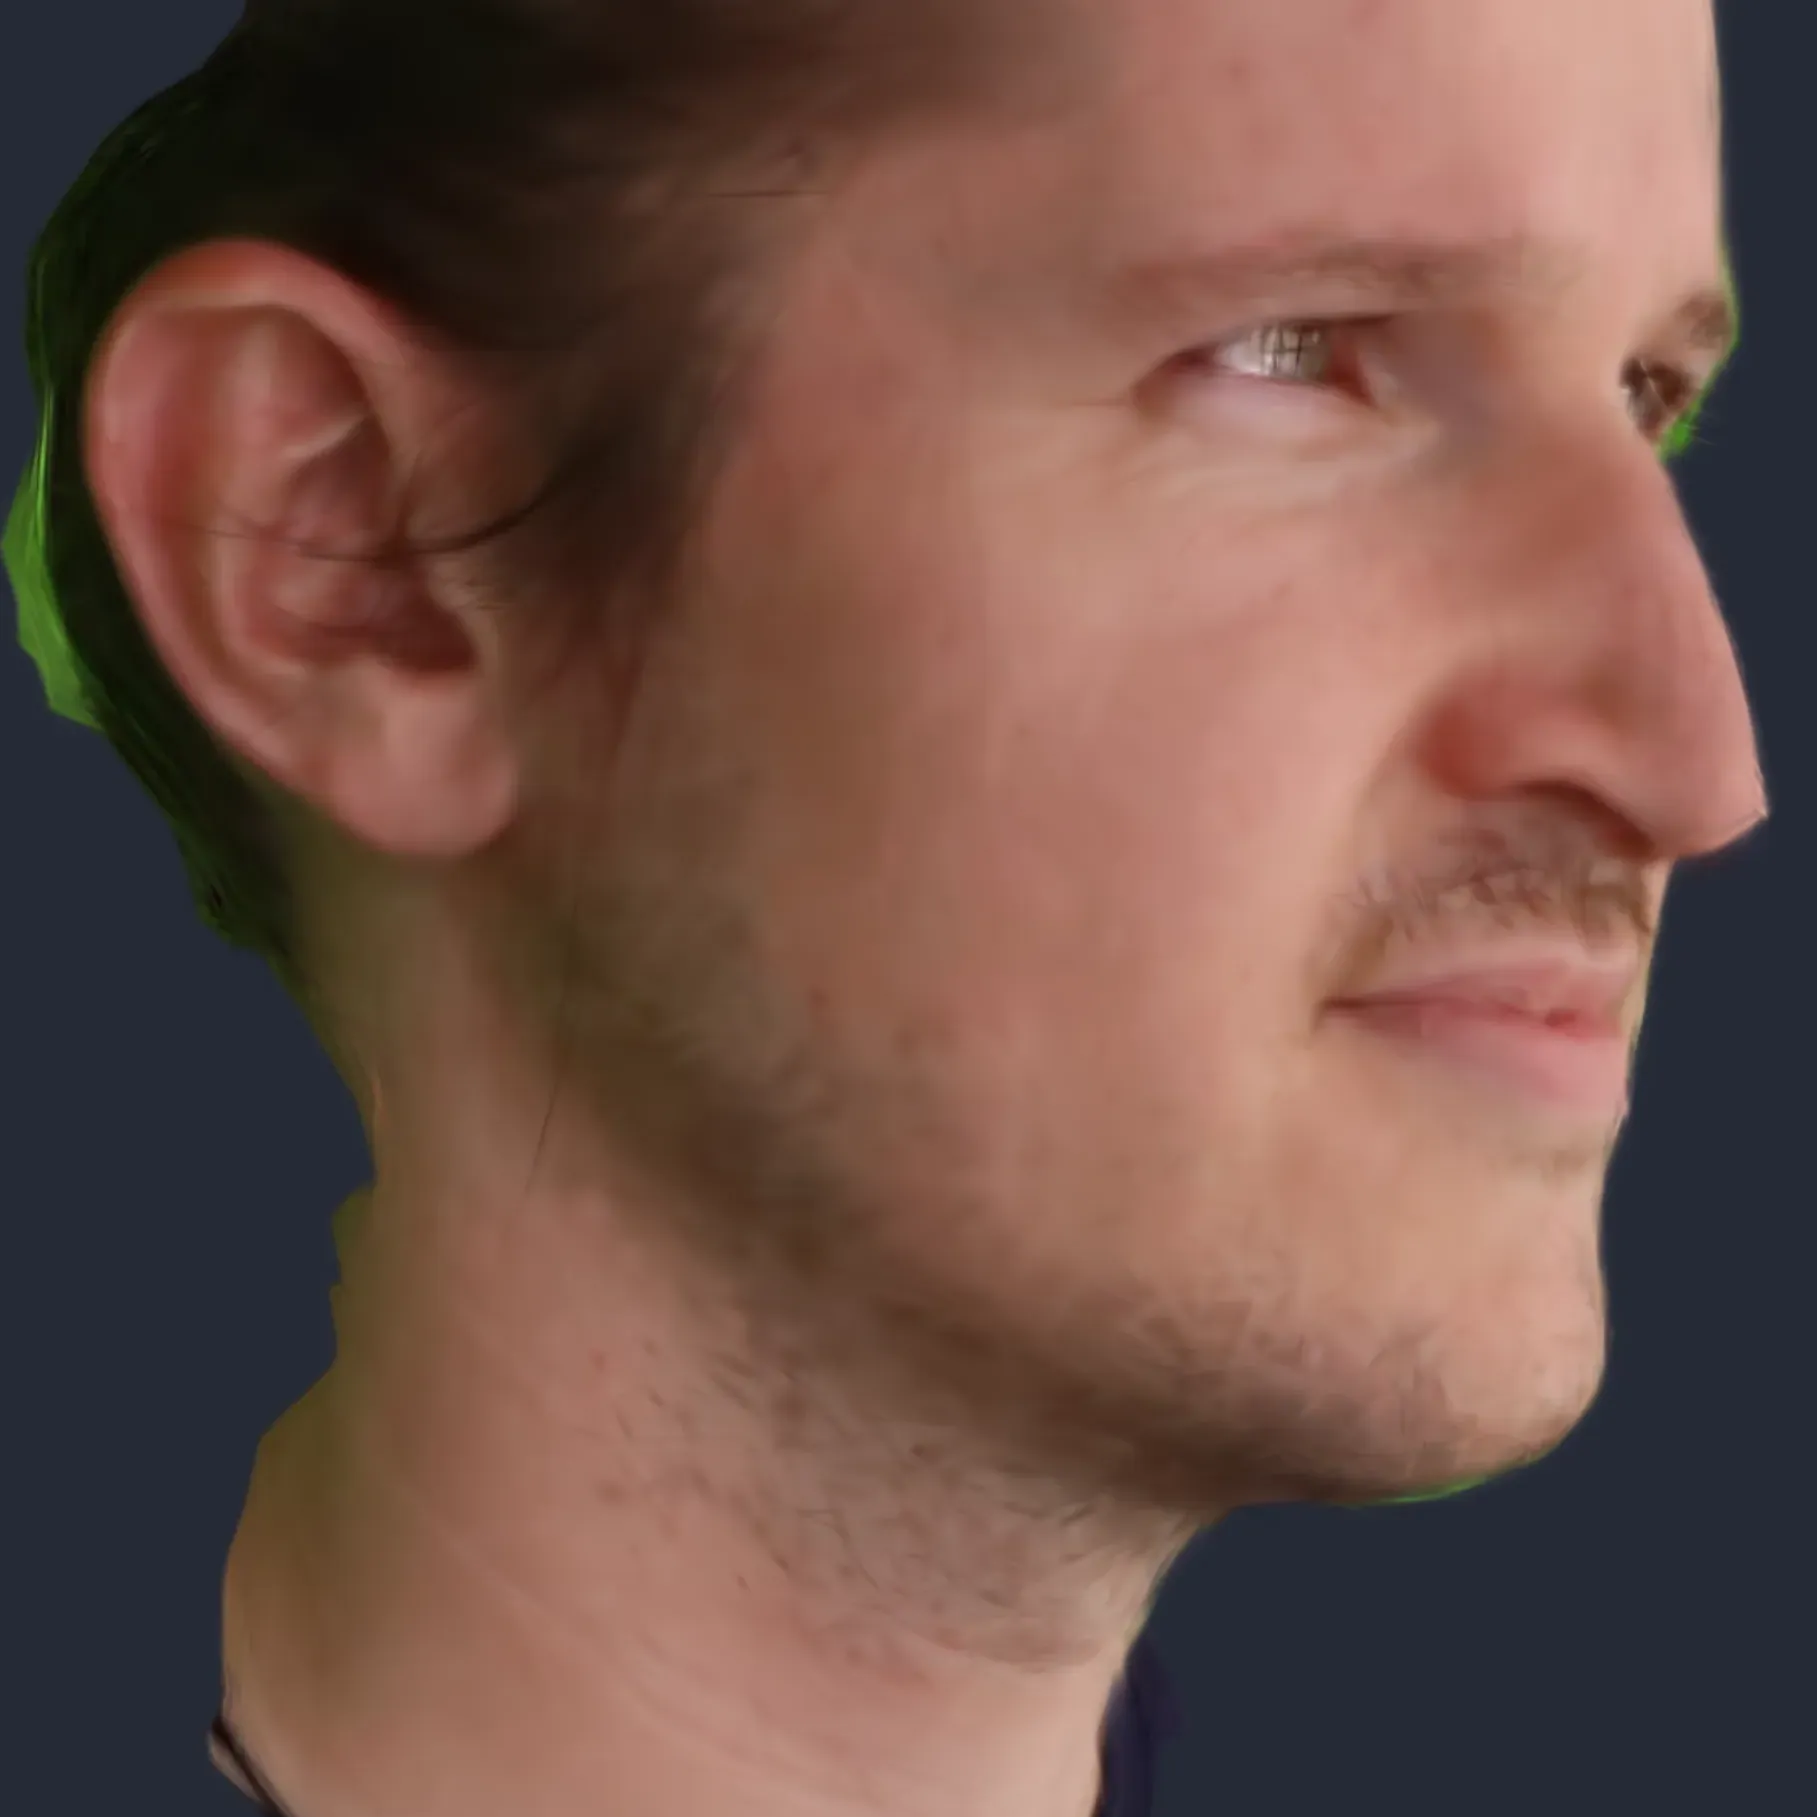
\includegraphics[width=\textwidth]{Figures/basics/rep5.png}
        \caption{3D Gaussian Splatting}
    \end{subfigure}
    \caption{Overview of different 3D representations.}
    \label{fig:3D_representation}
\end{figure}

\subsection{Meshes}

Polygonal meshes, often referred to simply as meshes, are among the most commonly used 3D models in computer applications. These meshes provide a structured representation of surfaces through a network of polygonal faces, typically triangles, interconnected by shared vertices and edges \citep{Shirley.2002}. The fundamental components of a triangle mesh are a set of triangles formed by vertex triplets, along with the 3D positions of these vertices.

Meshes can store additional data at vertices, edges, or faces to facilitate texture mapping, shading, animation, and other operations. Vertex data commonly includes material parameters, texture coordinates, and irradiance values. These parameters are interpolated across triangles to create a continuous function over the mesh's surface. The mesh resolution, determined by the number of polygons or triangles, dictates the mesh's detail level and surface smoothness. Meshes are widely used in computer graphics due to their simplicity, flexibility, and support in most 3D rendering applications.

Despite their utility, meshes are less suitable for deformation and style transfer tasks due to their complex topology and diverse data structures \citep{Kang.2023}. Current mesh style transfer approaches leverage differentiable rendering \citep{Kato.2018} to deform and optimize meshes based on input text prompts \citep{Michel.2021} or image styles \citep{Gao.2022}. However, these methods often struggle with satisfactory deformations due to complex topologies, insufficient mesh resolution, and gradient computation challenges in differentiable rendering \citep{Kato.2020}.


\subsection{Point Clouds}

Point clouds represent 3D objects as a set of discrete points in space, each defined by its position and potentially additional information such as color or surface normals. The density of these points influences the resolution, allowing different parts of the model to have varying levels of detail. Point clouds are commonly generated from 3D scanning of real-world objects or environments using specialized devices or photogrammetry software. Unlike meshes, point clouds lack connectivity between points, making them flexible and precise but less suitable for tasks like rendering and animation \citep{Bassier.2020}.
Direct style transfer on point clouds is less common \citep{Cao.2020}, with point clouds often serving as intermediate representations in 3D reconstruction processes, such as mesh reconstruction or implicit function representation \citep{Mildenhall.2020, Kerbl.2023, Mu.2021}.

\subsection{Neural Radiance Fields}
Neural Radiance Fields (NeRF) \citep{Mildenhall.2020} model 3D scenes as a 5D function mapping 3D coordinates and view directions to color and opacity values. Using a multilayer perceptron (MLP), NeRF reconstructs scenes from a set of 2D images captured from various viewpoints. The MLP is trained to predict color and opacity along camera rays, minimizing the error between rendered and actual pixel colors.

Once trained, NeRF can generate photorealistic views of scenes from novel angles. However, NeRF's computational demands make it unsuitable for real-time applications. NeRF lacks a geometric scene representation, limiting its use in interactive tasks like collision detection or animation. Conversion to mesh or point cloud representations, such as through Signed Distance Fields (SDF) \citep{Darmon.2021} or the Marching Cubes algorithm \citep{Lorensen.1987}, can address these limitations.


\subsection{3D Gaussian Splatting}

With 3D Gaussian Splatting \Citep{Kerbl.2023}, a scene is represented as a collection of many 3D Gaussians. These 3D Gaussian objects can be thought of as fuzzy blobs that collectively approximate the geometry and appearance of the scene. With sufficient density and overlap, a collection of 3D Gaussians can effectively visualize a surface reconstruction of a real-world object or scene with high accuracy. A 3D Gaussian is chosen because, unlike triangles in meshes or points, it is differentiable and enables backward and forward pass in a neural network. Consequently, a 3D Gaussian can be easily modified to fit the real-world scene during optimization using gradient descent. Each Gaussian $g$ is defined by the following parameters:

\begin{itemize}[noitemsep]
    \item Mean $\mu$: The position (center) of the Gaussian in 3D space.
    \item Covariance Matrix $\Sigma$: The orientation and anisotropy (shape) of the Gaussian.
    \item Alpha $ \alpha$: The opacity of the Gaussian.
    \item Spherical Harmonics $c$: The color of the Gaussian.
\end{itemize}

A scene of 3D Gaussian Splatting can be denoted as a collection of 3D Gaussians $G = \{g_0, g_1, \dots ,g_N\}$, where each individual Gaussian $g = \{\mu , \Sigma , c, \alpha \}$.

As seen in Figure \ref{fig:3D_Gaussian_Splatting}, the learning process starts with initialization using a set of image tie points via Structure from Motion (SfM). Initial 3D Gaussians are placed at these tie points. \textcolor{green}{Green} arrows indicate the forward process where the actual scene is rendered from a camera view. \textcolor{orange}{Orange} arrows indicate the gradient flow where the ground truth/training image is compared to the rendered image and reprojected to the 3D scene to update the 3D Gaussians based on the loss. Specifically, the 3D Gaussian Splatting scene is trained with a modified L1 loss containing a D-SSIM \citep{Baker.2023} term. This process is repeated for each camera view in the training data until the loss converges. 3D Gaussian Splatting is more efficient than NeRF because it does not require expensive ray sampling for rendering and instead uses a differentiable rasterizer.

\begin{figure}
    \centering
    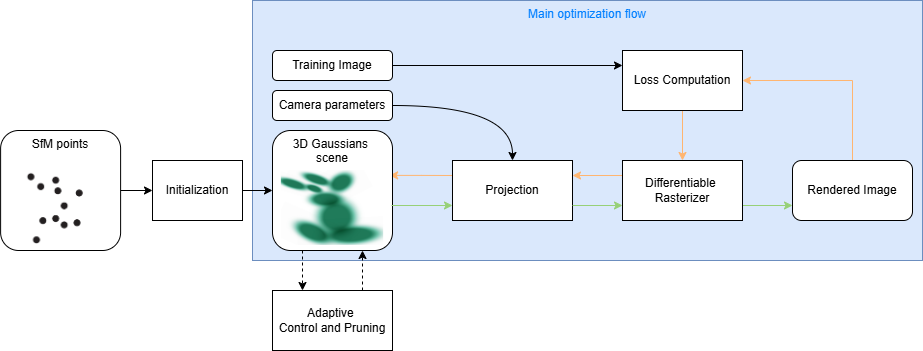
\includegraphics[width=\textwidth]{Figures/prelim_related/3D_gaussian_workflow.png}
    \caption{Overview of a 3DGS optimization process.}
    \label{fig:3D_Gaussian_Splatting}
\end{figure}

In addition, after every 100 iterations of the main optimization, a refinement process takes place. During this phase, the positioning and number of Gaussians in the scene are adaptively controlled to densely fit the scene's geometry and appearance, either by cloning, splitting, or moving them (indicated by the dotted arrow in Figure \ref{fig:3D_Gaussian_Splatting}). Furthermore, a pruning operation is carried out to cull or remove Gaussians with high transparency. As the optimization progresses, the Gaussians are refined, and the rendered image becomes more accurate based on the loss calculated from the difference between the rendered and ground truth images. The final result is a set of 3D Gaussians that represent the geometry and appearance of the scene.

\section{Image Style Transfer}

Image style transfer is a technique that allows one to transfer the style of one image to a content image. This technique is often used in computer vision to create stylized images and videos. The main idea behind image style transfer is to separate the content of an image from its style. The content of an image refers to the objects and their arrangement in the image, while the style of an image refers to the colors, textures, and patterns. By separating the content from the style, one can transfer the style of one image to a target image while preserving the content of the target image. This technique has been widely adopted in computer graphics to create stylized images and videos.

\subsection{Neural Style Transfer}

Pioneered by \textcite{Gatys.2015}, convolutional neural network (CNN)-based style transfer is a foundational technique for producing convincing artistic transformations beyond mere strokes and coloration changes. This approach, often called Neural Style Transfer (NST), employs a pre-trained CNN model, such as the Visual Geometry Group's VGG-19 network trained on the ImageNet dataset, to separate and recombine the content and style features of images. 

The content loss function $ \mathcal{L}_{content}$ is defined by the squared Euclidean distance between the feature representations of the content image $I_c$ and the generated image $I_g$ encoded by the VGG network at layer $l$ as follows:

\begin{equation}
    \mathcal{L}_{content} (I_c, I_g, l) = \frac{1}{2} \sum^{L}_{i,j} (VGG^{l}_{ci,j} -VGG^{l}_{gi,j} )^2
\end{equation}
where $VGG^l{ci,j}$ is the activation of the $i$-th convolution at the $j$-th position of layer $l$. The style loss exploits Gram-based visual texture modeling, defined by the squared Euclidean distance between the Gram-based style representations $\mathcal{G}$ from the VGG network for the style image $I_s$ and the generated image $I_g$:
\begin{equation}
    \mathcal{L}_{style} = \sum^{L}_{i,j} w_l \frac{1}{4N^2_l M^2_l} (\mathcal{G}^{l}_{ij} - \mathcal{G}^{l}_{ij})^2
\end{equation}
Combining with the content loss and the style loss across the layers, the  total loss is computed as follows:
\begin{equation}
    \mathcal{L}_{total}(I_s,I_c,I_g) = \alpha \mathcal{L}_{content}(I_c,I_g) + \beta \mathcal{L}_{style}(I_s,I_g)
\end{equation}
Here, $\alpha$ and $\beta$ are hyperparameters controlling the relative importance of content and style losses. The total loss $\mathcal{L}_{total}$ is minimized using gradient descent to generate the stylized image $I_g$.

Despite its foundational role, classical NST has limitations, including high computational cost and single-style optimization, requiring full re-optimization for each new style \Citep{Chen.2023}. More advanced methods have emerged to support multiple styles within a single network \Citep{Varlamova.2022}. However, NST often struggles to deeply understand the interplay between content and style, relying on separate optimization processes that may not capture this relationship comprehensively \Citep{Jing.2020}.

\subsection{Diffusion Models}

With the rising public interest in deep learning-based techniques, diffusion-based methods have garnered significant attention. One of the prominent approaches is the Latent Diffusion Model (LDM), first proposed by \textcite{Rombach.2022}. Stable Diffusion (SD) is implemented as a Latent Text-to-Image Diffusion pipeline, trained on text-image pair datasets to generate images from textual prompts or descriptions. Formally, an SD model samples a 3-channeled image $I \in \mathbb{R}^{3 \times H \times W}$ from a conditional distribution $p(I | y)$, where $y$ is the textual input prompt.

\begin{figure}[ht]
    \centering
    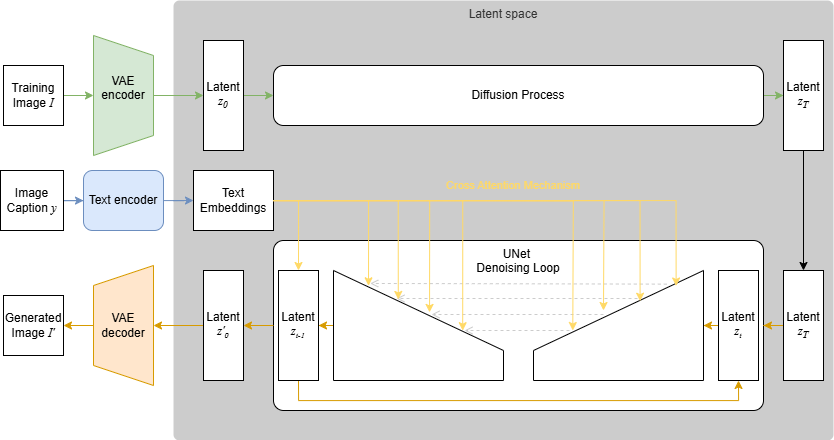
\includegraphics[width=0.8\textwidth]{Figures/prelim_related/sd-workflow.png}
    \caption{Simplified overview of the Stable Diffusion pipeline.}
    \label{fig:stable_diffusion}
\end{figure}

SD consists of three main components: a Variational Autoencoder (VAE), a U-Net architecture, and a conditioning encoder. The VAE encodes the image into a latent representation $z$ and decodes it back to an image. It is trained separately to compress the image into a much smaller latent space that captures its semantic features. The U-Net is a convolutional neural network responsible for image generation through the denoising of the latent space with the help of embeddings. The U-Net architecture is illustrated in Figure \ref{fig:controlnet}a. In the text-to-image generation SD pipeline, the conditioners are textual embeddings obtained by encoding textual descriptions using a Transformer language model, often CLIP \citep{Radford.2021}.

Training an SD model involves forward and backward propagation (illustrated by \textcolor{green}{green} and \textcolor{orange}{orange} arrows in Figure \ref{fig:stable_diffusion}). During forward propagation, a sample image $I$ is compressed into a latent representation $z$ to capture its semantic features using the VAE encoder $\mathcal{E}$, such that $z_0 = \mathcal{E}(I)$. Gaussian noise $x$ is then added at each step $t \in T$ according to a noise schedule $0 < \beta_1 < \dots < \beta_T < 1$ to produce a noisy latent $z_t = z + \beta_t$. At the last step $T$, the latent consists purely of Gaussian noise.

Backward propagation, where denoising occurs, iteratively reverts the latent $z_T$ to $z_0$ following the same schedule. The U-Net, conditioned on the textual embedding via a cross-attention mechanism (\textcolor{yellow}{yellow} arrow), predicts the total noise $\hat{\beta}_t$ in $z_t$ to estimate $z_0$. Since the predicted noise $\hat{\beta}_t$ is likely inaccurate, only a fraction $x$ of this noise is removed from $z_t$, such that $z_{t-1} = z_t - x \hat{\beta}_t$. This process repeats for every step $t$ until the loss converges. The aim is to optimize the noise distribution at each step by minimizing the loss between the predicted noise and the actual noise. This loss is computed as the negative log likelihood of the predicted noise given the actual noise. The process continues for all images in the dataset until convergence, with sampled images $I' \approx I$.

Using an SD model for text-to-image generation involves only the backward process, starting with pure Gaussian noise and gradually refining it using the user's text prompt as denoising guidance. The fully denoised latent is decoded via the VAE decoder to produce the final image.

Editing facial images with SD typically requires the face to occupy a large portion of the image. As shown in Figure \ref{fig:unpreprocessed}, stylizing Photodome images without sufficient preprocessing often leads to undesirable facial deformations or non-visible changes. This is because the model is trained on a dataset of images where faces are centered and occupy significant space. Consequently, the model struggles to generalize to images where faces are off-center or occupy a smaller area. This limitation can be mitigated by preprocessing images to center the face and crop them to the desired size before stylization. This challenge also applies to other SD pipelines like InstructPix2Pix \citep{Brooks.2023}, which will be discussed in the next section.

\begin{figure}
	\centering
	\begin{subfigure}{0.48\linewidth}
		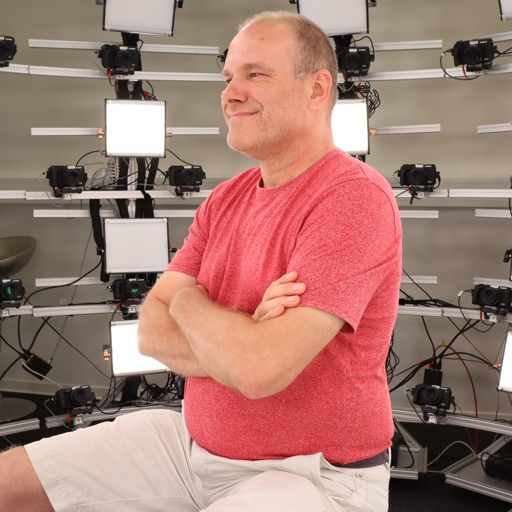
\includegraphics[width=\textwidth]{Figures/unpreprocessed/0-1-5-1-294_210300_834.JPG}
        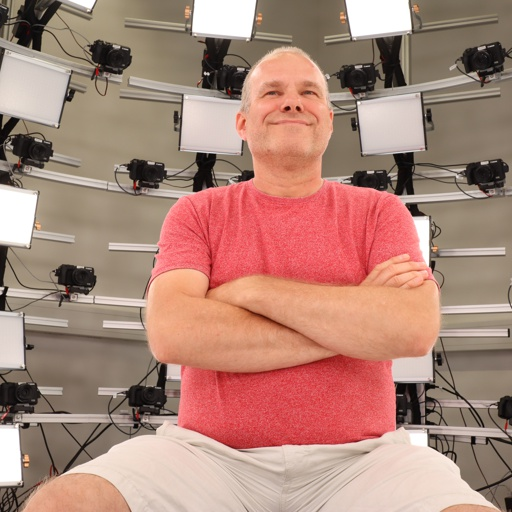
\includegraphics[width=\textwidth]{Figures/unpreprocessed/0-2-6-2-303_210300_871.JPG}
		\caption{Raw Photodome captures}
	\end{subfigure}
	\begin{subfigure}{0.48\linewidth}
		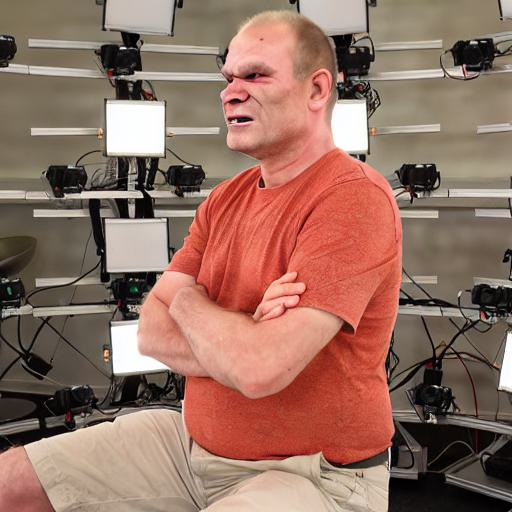
\includegraphics[width=\textwidth]{Figures/failed/sd_unprocessed/0-1-5-1-294_210300_834.JPG}
        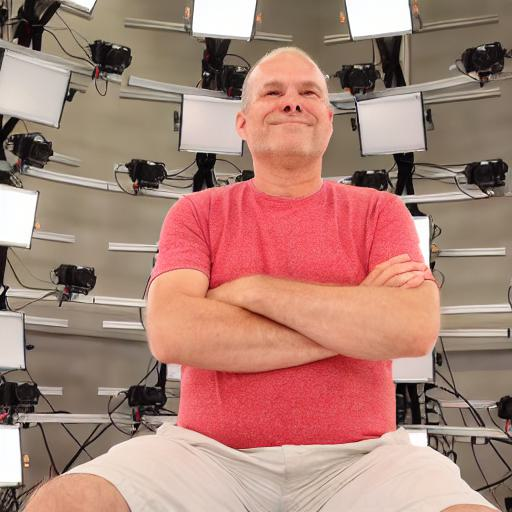
\includegraphics[width=\textwidth]{Figures/failed/sd_unprocessed/0-2-6-2-303_210300_871.JPG}
		\caption{"Photo of angry man"}
	\end{subfigure}
	\caption{Stylization of Photodome images without sufficient preprocessing steps tends to results in either undesirable facial deformation (top) or non-visible changes (bottom).}
	\label{fig:unpreprocessed}
\end{figure}

\subsubsection{InstructPix2Pix}
Today SD branches out from its original purpose to incorporate other technology in order to produce more convincing results or to accomplish different tasks. InstructPix2Pix \Citep{Brooks.2023} modifies the original SD model to enable image stylization using human instructions as opposed to the common text prompt used in the original SD model. This is done by training other SD model and usage of a Large Language Model (LLM) to generate several intermediate synthetic training datasets as seen in Figure \ref{fig:instructpix2pix}. To generate the initial dataset, \Textcite{Brooks.2023} first manually create 700 \textit{<source caption, target caption, edit instruction>} triplets, then leverage them to fine-tune a \textit{GPT-3} language model to make it generate a larger amount multi-modal synthetic dataset consisting of 454 thousand triplets. To transform the \textit{<source caption, target caption>} pairs into \textit{<source image, target image>} pairs, they use \textit{Prompt2Prompt}, a modified SD model \Citep{Hertz.2022} that enables intuitive text-based editing of real images with the SD model.
Finally, the \textit{<source image, target image, edit instruction>} triplets are used to fine-tune a SD model into the InstructPix2Pix model.
\begin{figure}[h]
    \centering
    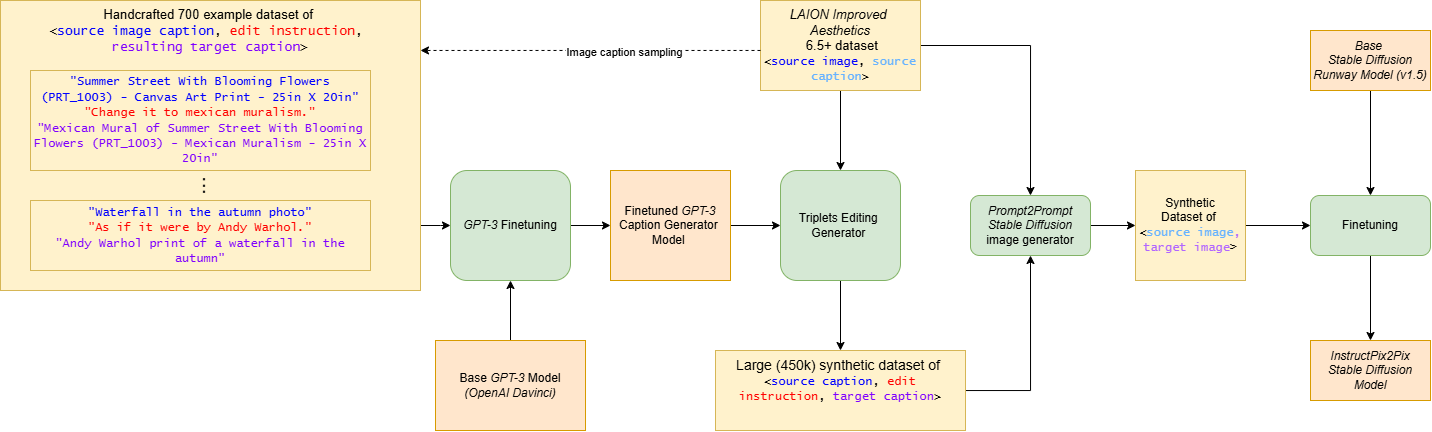
\includegraphics[width=0.8\textwidth]{Figures/prelim_related/instructpix2pix_training.png}
    \caption{Overview of InstructPix2Pix model training workflow.}
    \label{fig:instructpix2pix}
\end{figure}

Unlike other SD pipelines, InstructPix2Pix and Prompt2Prompt are considered style transfer techniques as they can plausibly transform an image by altering its content and style while preserving similarity to the original image, rather than being fully generative models. Figures \ref{fig:instructpix2pix_initial_4-5-1} and \ref{fig:instructpix2pix_initial_2-4-2} show experimental results of the InstructPix2Pix model from different view angles during the initial research, using two different configurations: default and modified guidance scales. By setting the lower textual guidance scale to 5 and the image guidance scale to 2, the model produces plausible results.

\begin{figure}[ht]
    \centering
    \begin{subfigure}{0.18\linewidth}
        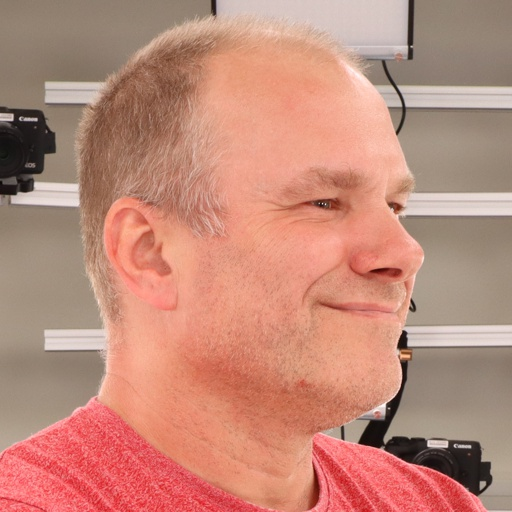
\includegraphics[width=\textwidth]{Figures/resized_images/0-4-5-1-5648_230239_266.JPG}
		\caption{Original}
	\end{subfigure}
    \begin{subfigure}{0.18\linewidth}
        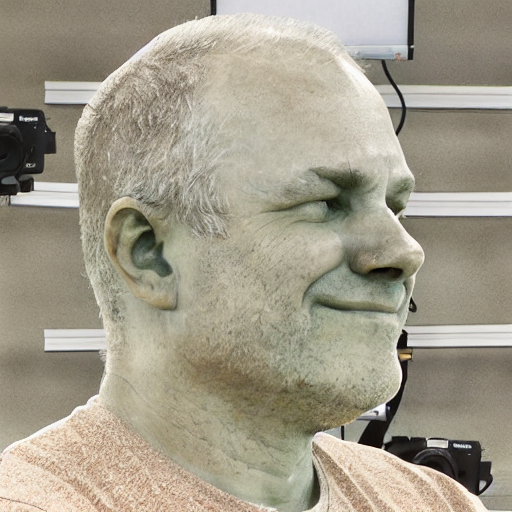
\includegraphics[width=\textwidth]{Figures/naive/default/ipix2pix_sven_stone/0-4-5-1-5648_230239_266.png}
        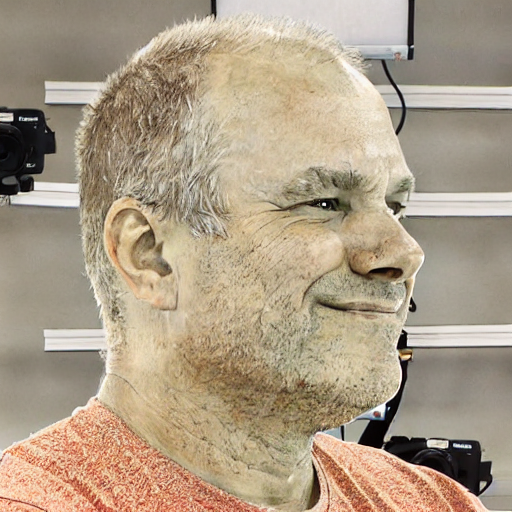
\includegraphics[width=\textwidth]{Figures/naive/low_cfg/ipix2pix_sven_stone/0-4-5-1-5648_230239_266.png}
    \caption{Stone statue}
	\end{subfigure}
    \begin{subfigure}{0.18\linewidth}
        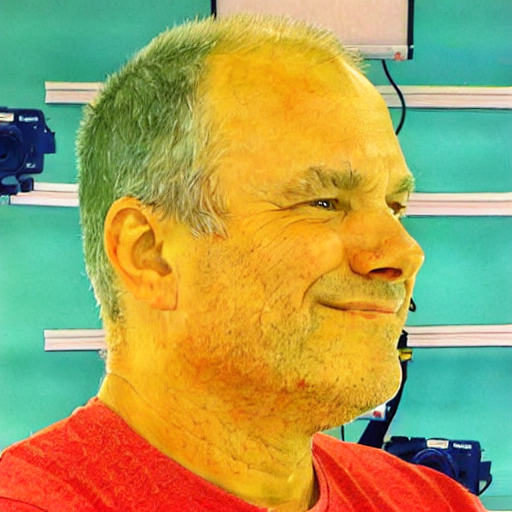
\includegraphics[width=\textwidth]{Figures/naive/default/ipix2pix_sven_fauvism/0-4-5-1-5648_230239_266.png}
        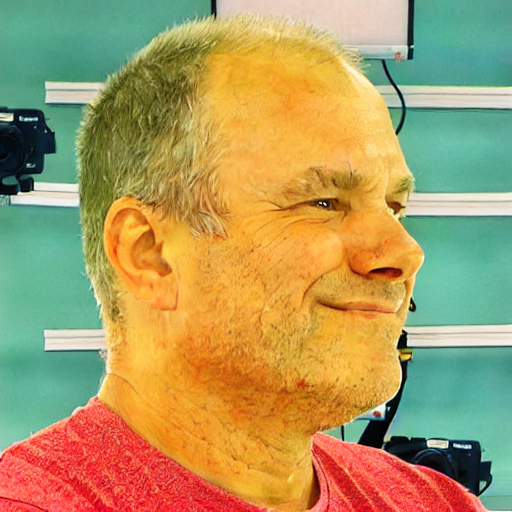
\includegraphics[width=\textwidth]{Figures/naive/low_cfg/ipix2pix_sven_fauvism/0-4-5-1-5648_230239_266.png}
        \caption{Fauvism}
	\end{subfigure}
    \begin{subfigure}{0.18\linewidth}
        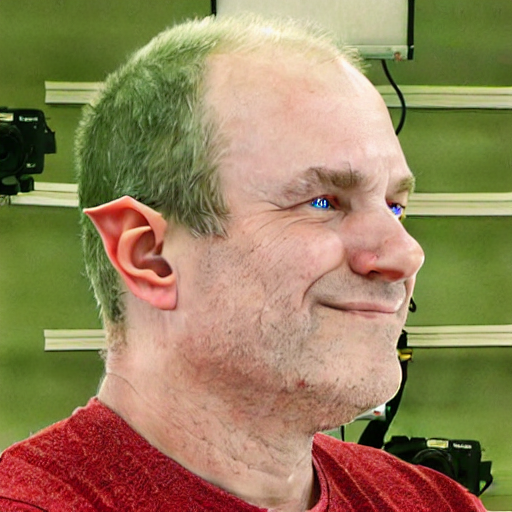
\includegraphics[width=\textwidth]{Figures/naive/default/ipix2pix_sven_elf/0-4-5-1-5648_230239_266.png}
        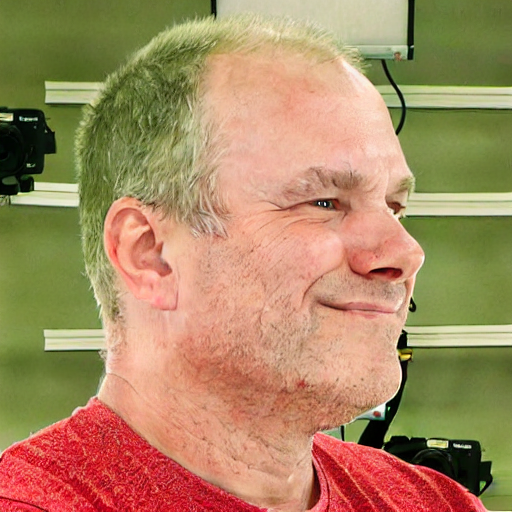
\includegraphics[width=\textwidth]{Figures/naive/low_cfg/ipix2pix_sven_elf/0-4-5-1-5648_230239_266.png}
        \caption{Tolkien elf}
	\end{subfigure}
    \begin{subfigure}{0.18\linewidth}
        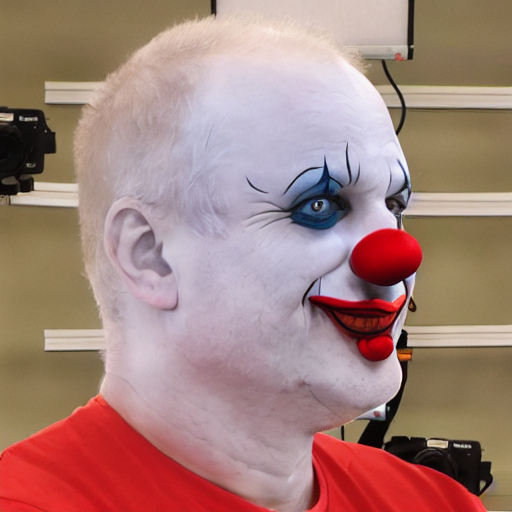
\includegraphics[width=\textwidth]{Figures/naive/default/ipix2pix_sven_clown/0-4-5-1-5648_230239_266.png}
        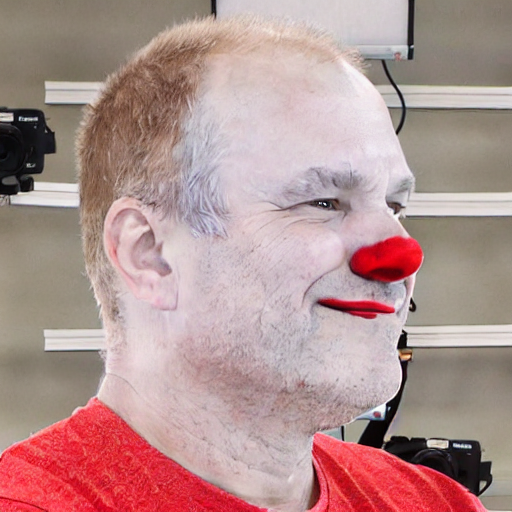
\includegraphics[width=\textwidth]{Figures/naive/low_cfg/ipix2pix_sven_clown/0-4-5-1-5648_230239_266.png}
		\caption{Clown}
	\end{subfigure}
    \caption{From camera 4-5-1, initial experimental test of the InstructPix2Pix model with various prompts. Top: results with default settings. Bottom: results with a low textual guidance scale.}
    \label{fig:instructpix2pix_initial_4-5-1}

\end{figure}

\begin{figure}
    \begin{subfigure}{0.18\linewidth}
        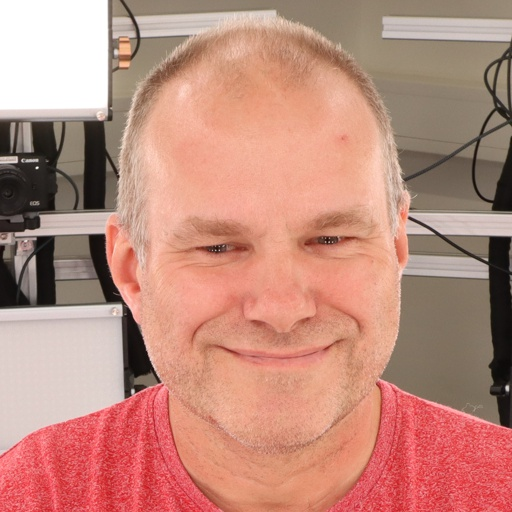
\includegraphics[width=\textwidth]{Figures/resized_images/0-2-4-2-293_210300_829.JPG}
		\caption{Original}
	\end{subfigure}
    \begin{subfigure}{0.18\linewidth}
        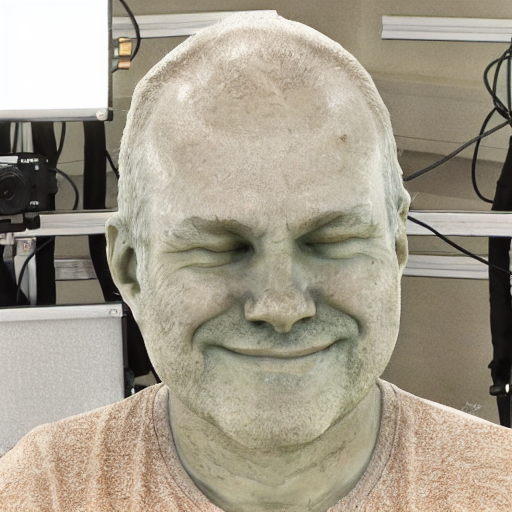
\includegraphics[width=\textwidth]{Figures/naive/default/ipix2pix_sven_stone/0-2-4-2-293_210300_829.png}
        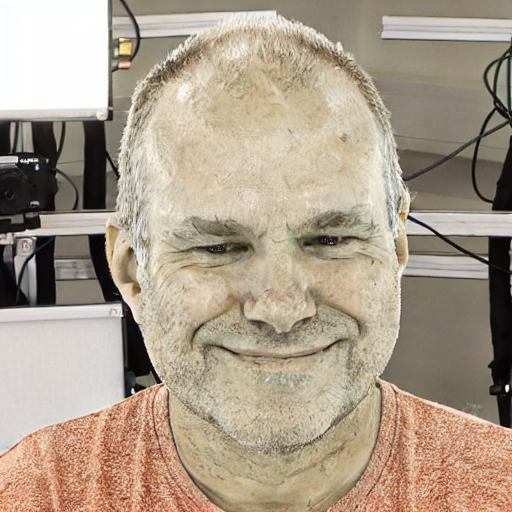
\includegraphics[width=\textwidth]{Figures/naive/low_cfg/ipix2pix_sven_stone/0-2-4-2-293_210300_829.png}
        \caption{Stone statue}
	\end{subfigure}
    \begin{subfigure}{0.18\linewidth}
        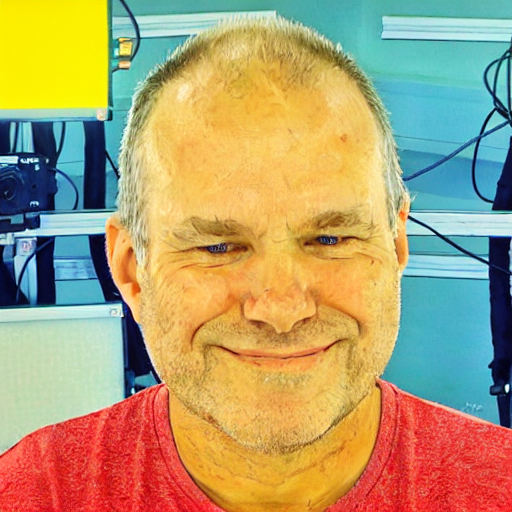
\includegraphics[width=\textwidth]{Figures/naive/default/ipix2pix_sven_fauvism/0-2-4-2-293_210300_829.png}
        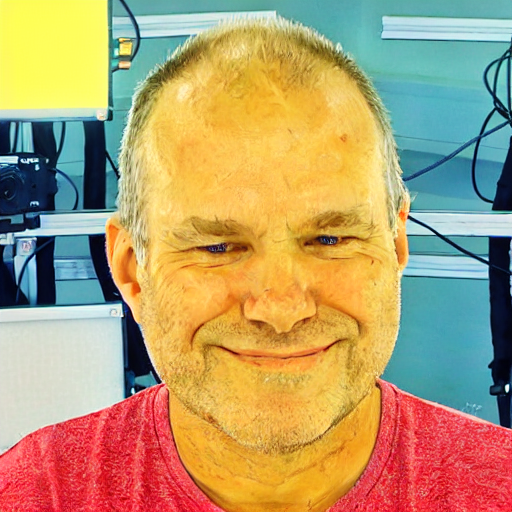
\includegraphics[width=\textwidth]{Figures/naive/low_cfg/ipix2pix_sven_fauvism/0-2-4-2-293_210300_829.png}
        \caption{Fauvism}
	\end{subfigure}
    \begin{subfigure}{0.18\linewidth}
        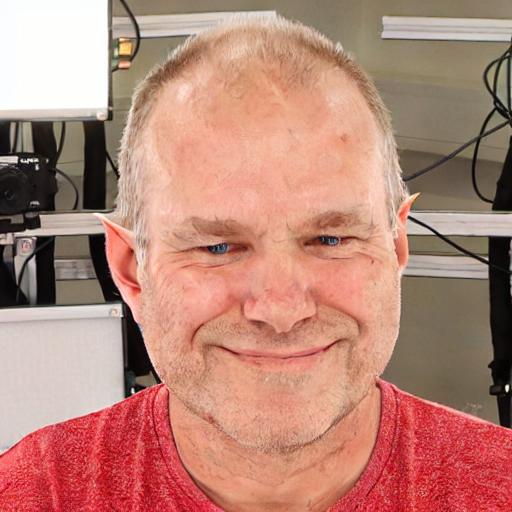
\includegraphics[width=\textwidth]{Figures/naive/default/ipix2pix_sven_elf/0-2-4-2-293_210300_829.png}
        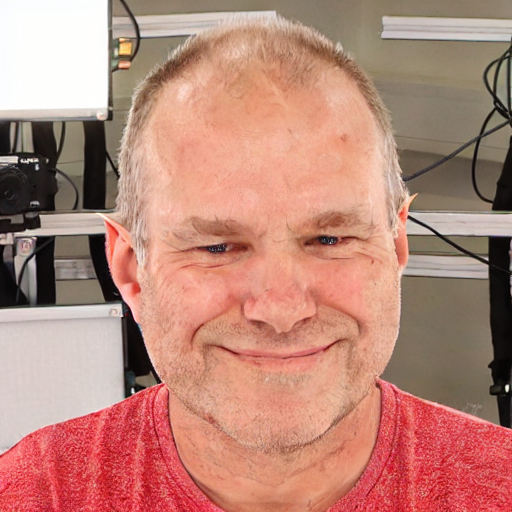
\includegraphics[width=\textwidth]{Figures/naive/low_cfg/ipix2pix_sven_elf/0-2-4-2-293_210300_829.png}
        \caption{Tolkien elf}
	\end{subfigure}
    \begin{subfigure}{0.18\linewidth}
        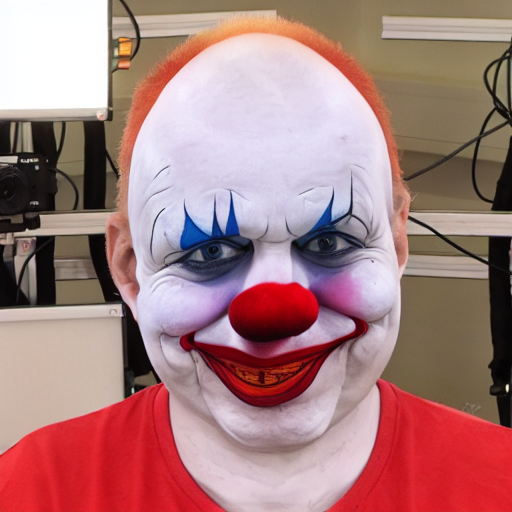
\includegraphics[width=\textwidth]{Figures/naive/default/ipix2pix_sven_clown/0-2-4-2-293_210300_829.png}
        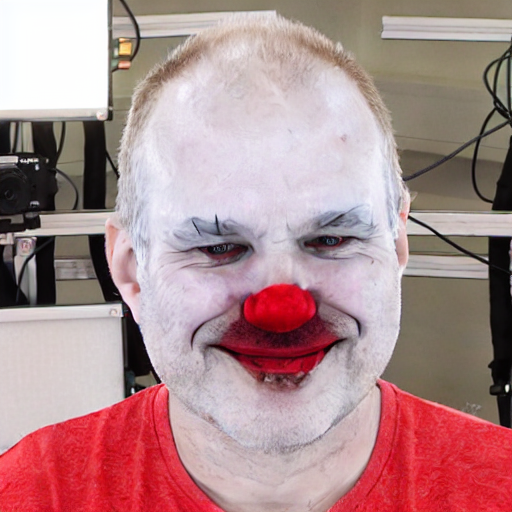
\includegraphics[width=\textwidth]{Figures/naive/low_cfg/ipix2pix_sven_clown/0-2-4-2-293_210300_829.png}
		\caption{Clown}
    \end{subfigure}
    \caption{From camera 2-4-2, initial experimental test of the InstructPix2Pix model with various prompts. Top: results with default settings. Bottom: results with a low textual guidance scale.}
    \label{fig:instructpix2pix_initial_2-4-2}

\end{figure}


\subsubsection{ControlNet}
Rather than retraining an SD model, \textcite{Zhang.2023} demonstrates that one can add a control network to a base SD pipeline to enable different conditioning inputs through ControlNet. ControlNet preserves the properties and capabilities of the base model by locking its parameters and adding a trainable copy of the default UNet encoding layers to the pipeline, as shown in Figure \ref{fig:controlnet}. As a result, conditional inputs such as depth maps, masks, edges, or poses can be applied to the original pipelines. Similar to text or conditioning images, these inputs are converted into latent representations and used as additional conditioners during the ControlNet-modified diffusion process. Consequently, the SD pipeline can perform more complex and diverse style transfer tasks. 

During the initial research for this thesis, ControlNet was found to be more generative in nature than editing, resulting in stylizations that barely resembled the original human face and often included facial deformations, particularly when combined with InstructPix2Pix. As shown in Figure \ref{fig:controlnet_failed}, stylization with ControlNet led to extreme alterations of the original even with several conditioners and a low textual guidance scale.

\begin{figure}[ht]
    \centering
    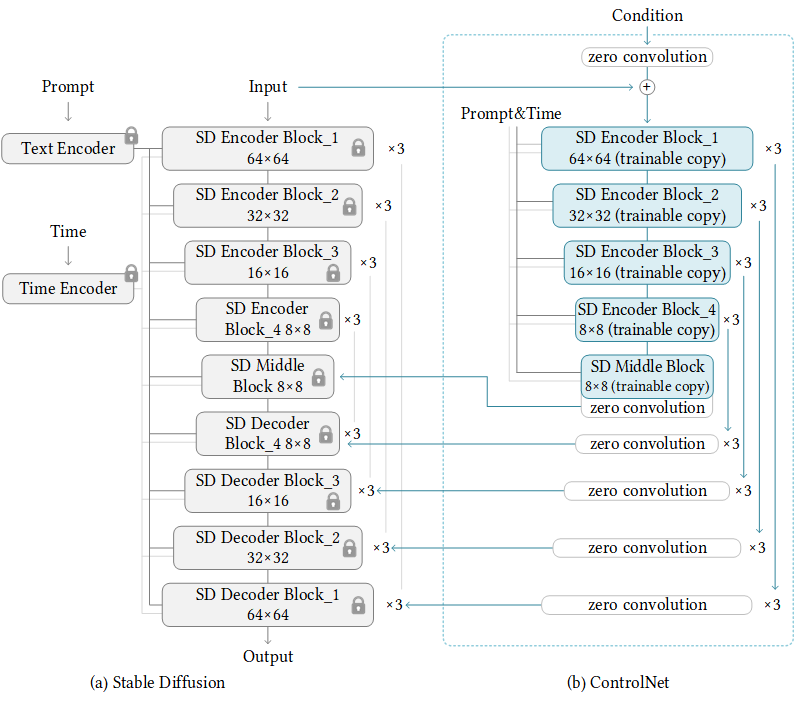
\includegraphics[width=0.7\textwidth]{Figures/prelim_related/controlnet.png}
    \caption{Comparison between the default UNet architecture of an SD pipeline (a) and ControlNet \citep{Zhang.2023} (b). In ControlNet, the attention mechanism is applied to the copy block instead of the main UNet block.}
    \label{fig:controlnet}
\end{figure}

Additionally, the random seed in ControlNet appears to have a larger impact on the results, particularly regarding their resemblance to the original inputs, compared to the original InstructPix2Pix pipeline. However, due to the popularity of this approach and SD in general, many contributors have published their versions of ControlNet with different architectures and training data. As such, this limitation may have been addressed in the latest versions of the pipelines and models.

\begin{figure}[ht]
    \centering
    \begin{subfigure}{0.18\linewidth}
        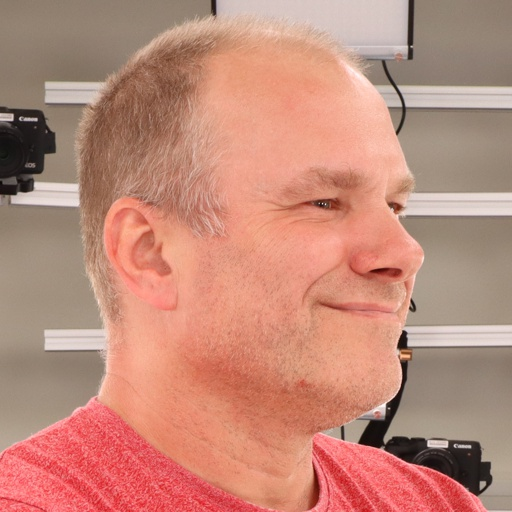
\includegraphics[width=\textwidth]{Figures/resized_images/0-4-5-1-5648_230239_266.JPG}
        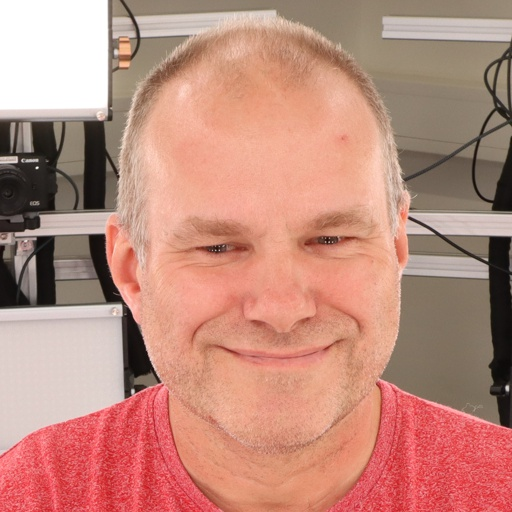
\includegraphics[width=\textwidth]{Figures/resized_images/0-2-4-2-293_210300_829.JPG}
        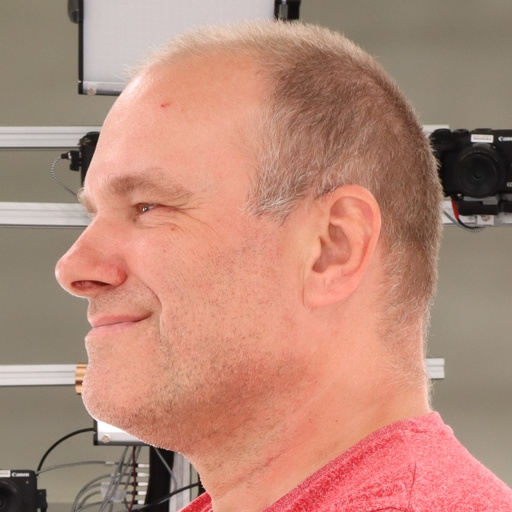
\includegraphics[width=\textwidth]{Figures/resized_images/0-C-5-1-5386_212530_574.JPG}
		\caption{Originals}
	\end{subfigure}
    \begin{subfigure}{0.18\linewidth}
        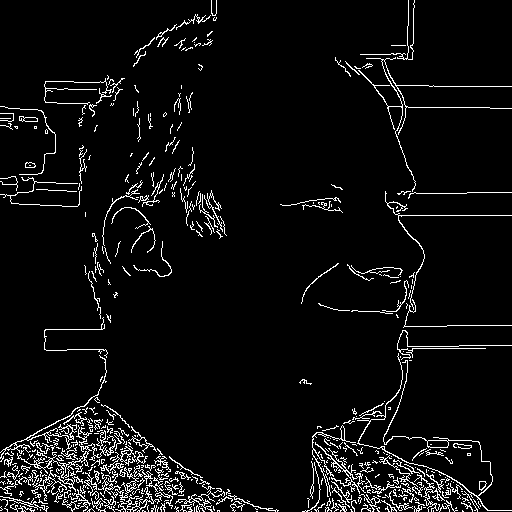
\includegraphics[width=\textwidth]{Figures/failed/controlnet/canny/0-4-5-1-5648_230239_266_canny.png}
        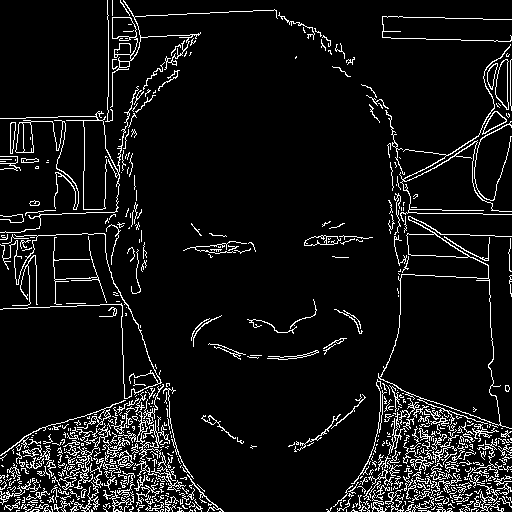
\includegraphics[width=\textwidth]{Figures/failed/controlnet/canny/0-2-4-2-293_210300_829_canny.png}
        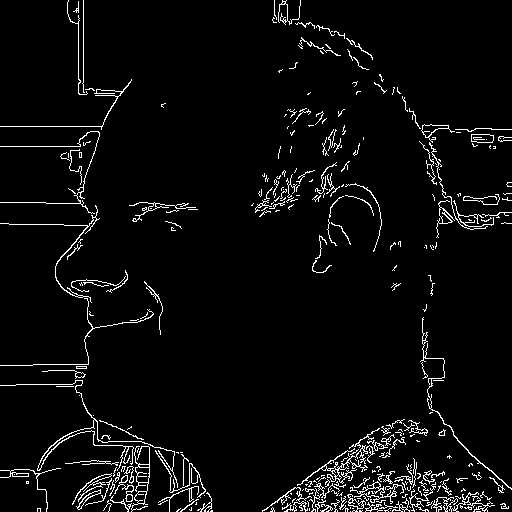
\includegraphics[width=\textwidth]{Figures/failed/controlnet/canny/0-C-5-1-5386_212530_574_canny.png}
		\caption{Canny edges}
	\end{subfigure}
    \begin{subfigure}{0.18\linewidth}
        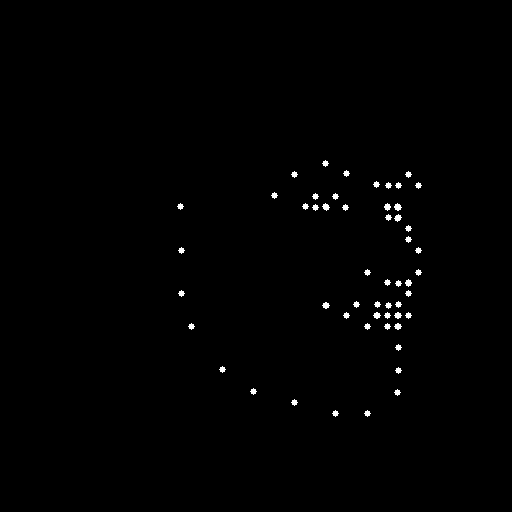
\includegraphics[width=\textwidth]{Figures/failed/controlnet/openpose/0-4-5-1-5648_230239_266_openpose.png}
        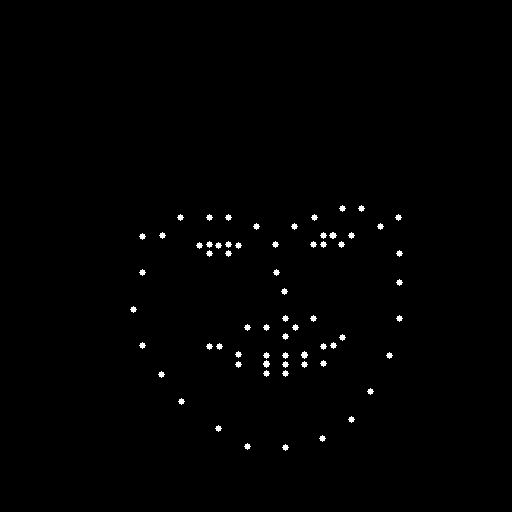
\includegraphics[width=\textwidth]{Figures/failed/controlnet/openpose/0-2-4-2-293_210300_829_openpose.png}
        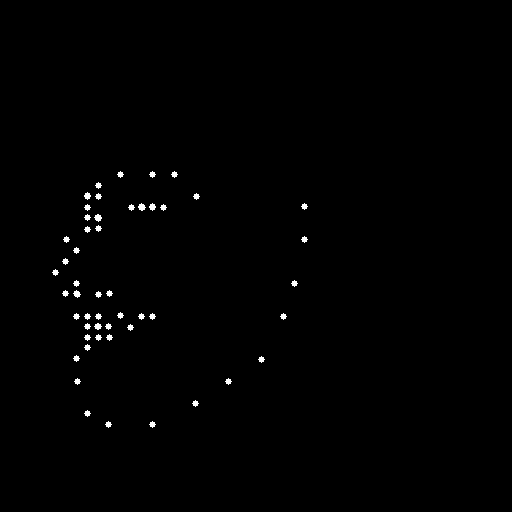
\includegraphics[width=\textwidth]{Figures/failed/controlnet/openpose/0-C-5-1-5386_212530_574_openpose.png}
        \caption{Face poses}
	\end{subfigure}
    \begin{subfigure}{0.18\linewidth}
        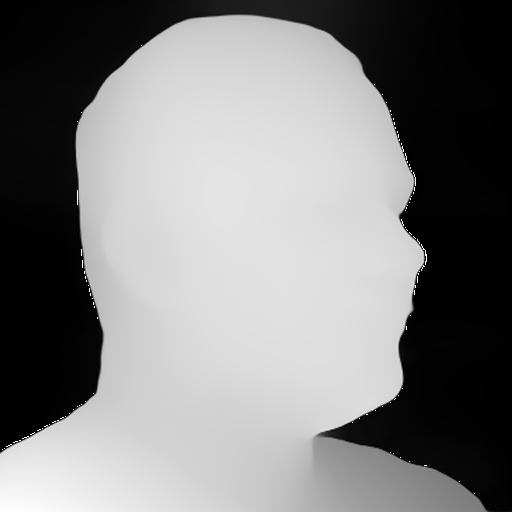
\includegraphics[width=\textwidth]{Figures/failed/controlnet/depth/0-4-5-1-5648_230239_266_depth.png}
        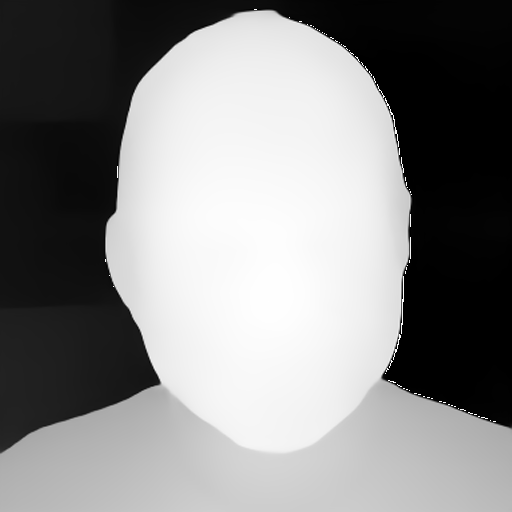
\includegraphics[width=\textwidth]{Figures/failed/controlnet/depth/0-2-4-2-293_210300_829_depth.png}
        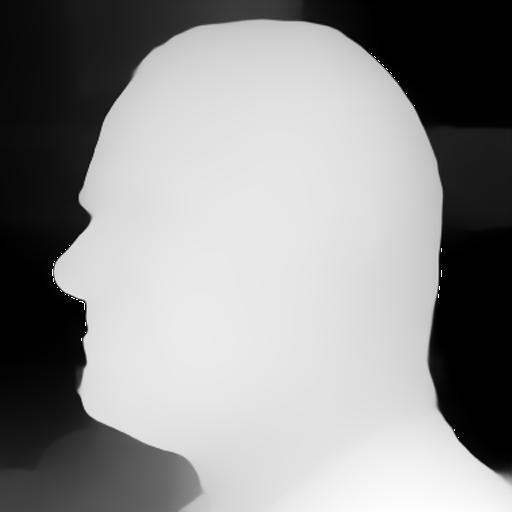
\includegraphics[width=\textwidth]{Figures/failed/controlnet/depth/0-C-5-1-5386_212530_574_depth.png}
        \caption{Depth maps}
	\end{subfigure}
    \begin{subfigure}{0.18\linewidth}
        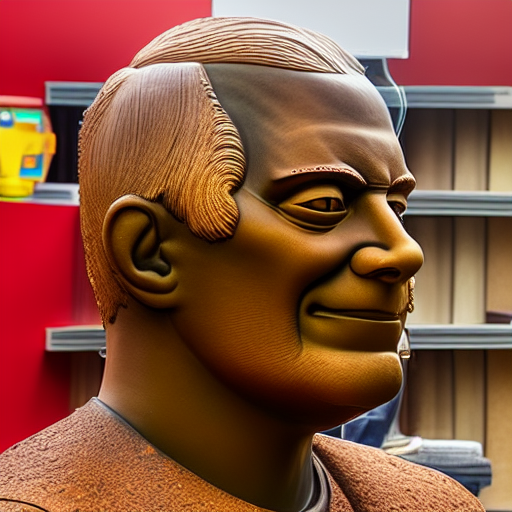
\includegraphics[width=\textwidth]{Figures/failed/controlnet/0-4-5-1-5648_230239_266.png}
        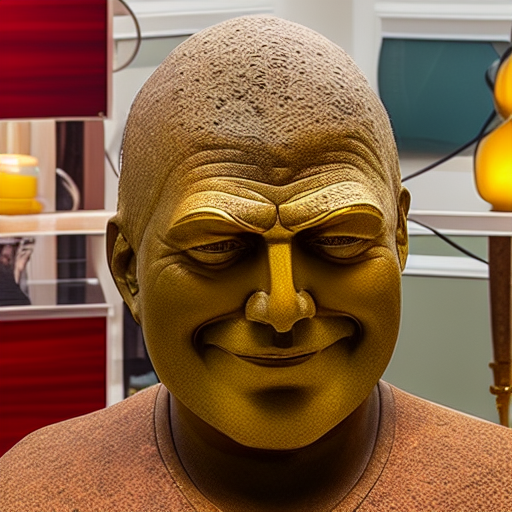
\includegraphics[width=\textwidth]{Figures/failed/controlnet/0-2-4-2-293_210300_829.png}
        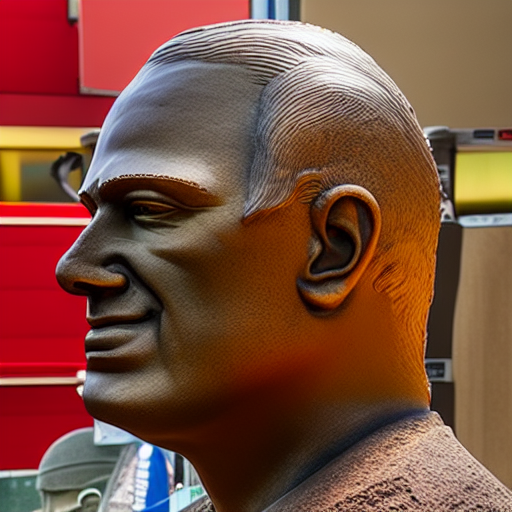
\includegraphics[width=\textwidth]{Figures/failed/controlnet/0-C-5-1-5386_212530_574.png}
		\caption{Results}
	\end{subfigure}
    \caption{Failed stylization results of ControlNet using the InstructPix2Pix pipeline with Canny edges, OpenPose for facial landmarks, and depth maps as conditioners, with the prompt "Turn him into a stone statue" and seed 33. Notice that the results not only barely resemble the original human face but also do not conform to the textual prompt.}
    \label{fig:controlnet_failed}
\end{figure}

\subsubsection{LoRa}

\textcite{Hu.2021} propose a novel fine-tuning method for pre-trained diffusion models called LoRa (Low-Rank Adaptation of Large Language Models). Traditionally, fine-tuning large language models such as GPT-3 is computationally expensive, as it requires updating all of the model's parameters. LoRa addresses this issue by introducing trainable low-rank decomposition matrices, which correspond to some of the base model's parameters. This allows for partial reparameterization of the model, significantly reducing the computational cost of fine-tuning. In the context of diffusion-based pipelines, LoRa has been used to modify the text encoders and/or denoising networks to emphasize (or de-emphasize) certain concepts or introduce new ones in the existing model. Building upon LoRa, \textcite{Yeh.2023} propose a new framework called LyCORIS (LoRa beYond Conventional methods, Other Rank adaptation Implementations) for diffusion-based models. This framework collects and analyzes various metrics and LoRa-based fine-tuning methods specifically for text-to-image generative models.

\section{Losses and metrics}

\subsection{$\mathcal{L}_1$ Loss}
The $\mathcal{L}_1$ loss, also known as mean absolute error (MAE), is a common loss function used in image processing tasks like image denoising, super-resolution, or image reconstruction. In the 2D domain, $\mathcal{L}_1$ loss is computed as the average of the absolute differences between each pixel in the predicted image and the corresponding pixel in the ground truth (original) image. It measures the difference between the predicted pixel values of an image and the true pixel values in a straightforward, absolute manner. The $\mathcal{L}_1$ loss is formulated as:
\begin{equation}
    \label{}
    \mathcal{L}_1(I_{pred},I_{true} ) = \frac{1}{N}  \sum ^N_{i = 1} | I_{pred}(i) - I_{true}(i)|
\end{equation}
where $N$ is the total number of pixels in the image, $I_{pred}(i)$ and $I_{true}(i)$ are the predicted and ground truth pixel values at location $i$, respectively. In the context of 3D stylization, $\mathcal{L}_1$ quantifies the difference between the expected stylization result and the actual stylized rendering of the 3D object.

\subsection{PSNR}
Peak Signal-to-Noise Ratio (PSNR) is a logarithmic measure that compares the maximum possible pixel value of an image (signal) to the difference (noise) between the original image and the distorted or reconstructed image. Mathematically, PSNR is defined as:

\begin{equation}
    PSNR(I_{pred},I_{true} ) = 10 \cdot \log_{10} (\frac{MAX_I^2}{\mathcal{L}_1(I_{pred},I_{true} )})
\end{equation}
where $MAX_I$ is the maximum possible pixel value of the image.

PSNR is widely used to assess the quality of lossy image compression methods like JPEG, and in other tasks such as image denoising, restoration, and super-resolution. In the 3D domain, PSNR serves as a quantitative metric to evaluate the quality of the reconstructed 2D views compared to the ground truth 2D views captured from a real-world object or scene. It can also evaluate the stylization quality of a 3D object from a camera view given the corresponding stylized image.

PSNR values are measured in decibels (dB). A typical good-quality image will have a PSNR value between 30–50 dB, where values above 40 dB are considered excellent.

\subsection{SSIM and DSSIM}

The DSSIM loss is derived from the SSIM (Structural Similarity Index), which compares two images based on structural information like luminance, contrast, and structure \citep{Wang.2004, Nilsson.2020}. SSIM aims to capture the human visual system's perception of similarity rather than simply relying on pixel-level differences. DSSIM measures the dissimilarity between images. In the context of image stylization, SSIM and DSSIM quantify the perceived similarity of the stylized image compared to the expected result.

\subsubsection{SSIM}
The SSIM formula comprises luminance, contrast, and structural components:
\begin{equation}
    \mathsf{SSIM}(I_{pred}, I_{true}) = l(I_{pred}, I_{true})^\alpha \cdot c(I_{pred}, I_{true})^\beta \cdot s(I_{pred}, I_{true})^\gamma
\end{equation}
where $l(I_{pred}, I_{true})$ is the luminance difference, $c(I_{pred}, I_{true})$ is the contrast difference, and $s(I_{pred}, I_{true})$ is the structural difference between the predicted image $I_{pred}$ and the ground truth $I_{true}$. The parameters $\alpha$, $\beta$, and $\gamma$ are weights for the contribution of each component.

The luminance, contrast, and structure components are defined as:
\begin{equation}
    l(I_{pred}, I_{true}) = \frac{2\mu_{pred}\mu_{true} + c_1}{\mu_{pred}^2 + \mu_{true}^2 + c_1}
\end{equation}

\begin{equation}
    c(I_{pred}, I_{true}) = \frac{2\sigma_{pred}\sigma_{true} + c_2}{\sigma_{pred}^2 + \sigma_{true}^2 + c_2}
\end{equation}

\begin{equation}
    s(I_{pred}, I_{true}) = \frac{\sigma_{pred, true} + c_3}{\sigma_{pred} \sigma_{true} + c_3}
\end{equation}

Here, $\mu_{pred}$ and $\mu_{true}$ are the pixel sample means of the predicted and ground truth images, respectively, denoting luminance. $\sigma_{pred}$ and $\sigma_{true}$ are the standard deviations, representing contrast. $\sigma_{pred, true}$ is the covariance between the images, denoting structure. Constants $c_1$, $c_2$, and $c_3$ are variables to stabilize the division when the denominator is weak.

\subsubsection{DSSIM}
To convert SSIM into a dissimilarity measure for use as a loss function, DSSIM is defined as:

\begin{equation}
    \mathsf{DSSIM}(I_{pred}, I_{true}) = \frac{1-SSIM(I_{pred}, I_{true})}{2}
\end{equation}

DSSIM is commonly used in tasks like image super-resolution, denoising, and style transfer, where structural integrity is crucial. In 3D stylization, DSSIM is particularly relevant when using 2D multi-view priors, as inconsistencies in stylization can compromise the quality of the resulting 3D object.

\subsection{CLIP Similarity Metrics}
CLIP (Contrastive Language-Image Pre-training) \citep{Radford.2021} is a convolutional neural network model developed by OpenAI that relates text and images in a shared embedding space. Several types of similarities can be computed using CLIP to measure relationships between text and images or between images themselves. Some uses of CLIP include Text-to-Image Direction Similarity (CTIDS) and Image-Image Similarity (CIIS).

\subsubsection{Text-to-Image Direction Similarity}
CLIP Text-Image Direction Similarity (CTIDS) measures how closely the semantic direction implied by a text prompt matches the direction between two images in CLIP's embedding space. It compares the vector direction from one image to another with the vector direction from a text prompt to one of the images. This measure is useful for evaluating how well a textual description captures the semantic change between two images.

\subsubsection{Image-Image Similarity}
CLIP Image-Image Similarity (CIIS) measures the similarity between two images purely based on their visual content as encoded in CLIP's image embedding space. CLIP embeds images into a vector space where visually and semantically similar images are positioned closer together. Image-Image Similarity is typically computed using cosine similarity between these image embeddings. The closer the cosine similarity is to 1, the more similar the images are. This is particularly useful for comparing multi-view images in the dataset and assessing the consistency of their stylization.

\subsection{FID}
FID (Fréchet Inception Distance) is a metric used to assess the quality of generated images by comparing them to a set of real images. In the context of image stylization, FID measures how closely the stylized images match the distribution of the original content or real-world images. It is particularly useful for evaluating generative models, such as style transfer networks, to assess how realistic and stylistically coherent the generated (stylized) images are, as well as how well the content of the real image is preserved in the stylized image. Lower FID indicates that the distribution of stylized images is closer to the original image distribution or the target style's distribution, implying better stylization quality and higher content preservation.

FID is computed using the following formula:
\begin{equation}
    FID = ||\mu_{real} - \mu _{style} + \mathsf{Tr} (\Sigma _{real} + \Sigma _{style} - 2(\Sigma_{real} \Sigma_{style} )^\frac{1}{2})
\end{equation}
where $\mu_{real}$ and $\mu_{style}$ are the means of the real (original) and generated (stylized) images' feature representations, $\Sigma_{real}$ and $\Sigma_{style}$ are the covariance matrices of the real and generated images' feature representations, and $\mathsf{Tr}$ is the trace of a matrix (the sum of its elements on the main diagonal).

\subsection{LPIPS}
LPIPS (Learned Perceptual Image Patch Similarity) \citep{Zhang.2018} is a perceptual similarity metric that measures the similarity between two images based on their perceptual features. LPIPS is designed to capture the perceptual similarity between images as perceived by humans. It uses deep features from various pre-trained deep neural networks, such as VGG or AlexNet, to serve as the basis of the metric, providing a closer correspondence to human perception of similarity than classical metrics like SSIM.

LPIPS is particularly useful for evaluating image quality in cases where spatial ambiguities are a factor. It is computed by comparing the perceptual features of two images using a pre-trained deep neural network. Lower LPIPS values indicate higher perceptual similarity between the images. However, there is no clearly defined upper bound. During initial research, it was observed that two completely different images could have an LPIPS value around 0.6. Moreover, no known documentation clarifies how LPIPS values scale in terms of image quality or similarity.

